% \iffalse
\let\negmedspace\undefined
\let\negthickspace\undefined
\documentclass[journal,12pt,twocolumn]{IEEEtran}
\usepackage{cite}
\usepackage{amsmath,amssymb,amsfonts,amsthm}
\usepackage{algorithmic}
\usepackage{graphicx}
\usepackage{textcomp}
\usepackage{xcolor}
\usepackage{txfonts}
\usepackage{listings}
\usepackage{enumitem}
\usepackage{mathtools}
\usepackage{gensymb}
\usepackage{comment}
\usepackage[breaklinks=true]{hyperref}
\usepackage{tkz-euclide}
\usepackage{listings}
\usepackage{gvv}
\def\inputGnumericTable{}
\usepackage[latin1]{inputenc}
\usepackage{color}
\usepackage{array}
\usepackage{longtable}
\usepackage{calc}
\usepackage{multirow}
\usepackage{hhline}
\usepackage{ifthen}
\usepackage{lscape}

\newtheorem{theorem}{Theorem}[section]
\newtheorem{problem}{Problem}
\newtheorem{proposition}{Proposition}[section]
\newtheorem{lemma}{Lemma}[section]
\newtheorem{corollary}[theorem]{Corollary}
\newtheorem{example}{Example}[section]
\newtheorem{definition}[problem]{Definition}
\newcommand{\BEQA}{\begin{eqnarray}}
\newcommand{\EEQA}{\end{eqnarray}}
\newcommand{\define}{\stackrel{\triangle}{=}}
\theoremstyle{remark}
\newtheorem{rem}{Remark}
\begin{document}

\bibliographystyle{IEEEtran}
\vspace{3cm}

\title{NCERT Discrete - 10.5.2.19}
\author{EE23BTECH11007 - Aneesh Kadiyala$^{*}$% <-this % stops a space
}
\maketitle
\newpage
\bigskip

\renewcommand{\thefigure}{\theenumi}
\renewcommand{\thetable}{\theenumi}
%fi
\vspace{3cm}
\textbf{Question 10.5.2.19:} Subba Rao started work in 1995 at an annual salary of Rs. 5000 and received an increment of Rs. 200 each year. In which year did his income reach Rs. 7000?

\solution
\begin{tabular}{ | c | c | c | }
    \hline
    Parameter & Value & Description \\
    \hline
    $x(0)$ & 30 & Initial no. of bacteria\\
    \hline
    $r$ & 2 & Ratio of no. of bacteria at end of \\
    & & hour to start of hour (Common Ratio) \\
    \hline
    $x(n)$ & $r^nx(0)u(n)$ & $n^{th}$ term of the GP \\
    \hline
\end{tabular} 
From the values given in \tabref{tab:1}:
\begin{align}
7000 &= 5000 + 200n \\
\implies 2000 &= 200n \\
\therefore n &= 10
\end{align}
\begin{align}
x(n) = (x(0) + nd)(u(n))
\end{align}
\begin{figure}[h!]
    \centering
    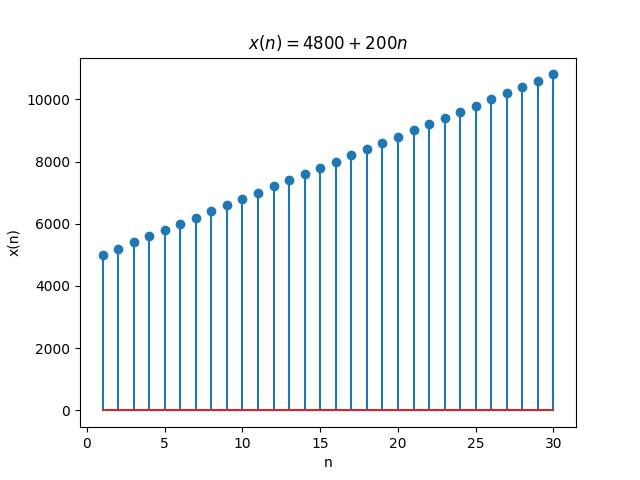
\includegraphics[width=\columnwidth]{figs/10_5_2_19.png}
    \caption{Plot of $x(n)$ vs $n$. See \tabref{tab:1} for details.}
    \label{fig:1}
\end{figure}
Let Z-transform of $x(n)$ be $X(z)$. Let $U(z)$ be the Z-transform of $u(n)$.
\begin{align}
X(z) &= \frac{x(0)}{1 - z^{-1}} + \frac{dz^{-1}}{(1 - z^{-1})^2} \quad |z| > 1
\end{align}
Using the values from \tabref{tab:1}:
\begin{align}
X(z) &= \frac{5000}{1 - z^{-1}} + \frac{200z^{-1}}{(1 - z^{-1})^2} \quad |z| > 1
\end{align}
\end{document}